\section*{选题价值}

随着智慧城市和智能交通的发展,行人导航与控制系统在现代交通管理中起到了重要作用。行人作为城市交通系统中不可或缺的参与者,其行为具有显著的随机性和多样性,这为传统的交通管理和路径规划方法带来了诸多挑战。行人导航系统的研究目标在于通过实时路径优化与智能调控,提升行人的交通安全与出行效率。然而,传统的导航方法多基于规则模型,主要依赖于静态预设参数,难以应对复杂动态环境中行人行为的快速变化。例如,面对突发的障碍物或密集的交通流动,传统算法往往无法快速调整路径规划或实时优化决策,从而影响导航系统的可靠性与安全性。

近年来,随着人工智能技术的快速发展,强化学习(Reinforcement Learning, RL)作为一种基于数据驱动的决策优化方法,为行人导航领域提供了全新的解决思路。强化学习通过智能体与环境的交互学习最优策略,能够在动态环境中实现实时决策优化,特别适用于非线性、非结构化的复杂场景。然而,仅依靠强化学习技术不足以全面解决行人导航问题,因为现实环境中的数据采集具有高成本、高风险的特点,这在实际应用中极大地限制了强化学习的训练与推广。

虚幻引擎(Unreal Engine)作为一种高仿真度的虚拟场景构建平台,提供了一个解决实际环境数据采集困难的理想工具。虚幻引擎不仅能够生成复杂多样的动态环境,还可以模拟真实场景中行人行为的随机性和多样性,为强化学习智能体的训练与测试提供了安全、低成本的实验平台。例如,通过虚幻引擎模拟十字路口的复杂交通场景,可以逼真再现行人与车辆之间的动态交互,为强化学习算法的优化与验证创造了实验条件。此外,虚幻引擎还支持多种传感器数据的生成,例如视觉、惯性和语义信息,进一步丰富了强化学习的训练数据来源。

结合虚拟仿真技术和强化学习算法,本研究旨在解决行人导航中的以下核心问题:

1. \textbf{ 动态环境下行人行为的精准建模:} 行人行为受到多种因素的影响,包括交通信号、周围车辆的动态变化以及其他行人的行为。如何建立一个高精度的行人行为模型,能够真实反映不同环境中行人的决策逻辑,是行人导航研究的首要难题。

2. \textbf{ 虚拟仿真与强化学习的高效结合:} 强化学习的有效性高度依赖于训练环境的质量,而虚幻引擎的仿真能力为训练高效的智能体提供了可能。然而,如何设计高效的强化学习算法,充分利用虚幻引擎生成的多样化数据,仍然是一个亟待解决的问题。

3. \textbf{ 平衡路径规划的效率与行人安全性:} 行人导航系统不仅需要提高路径规划的效率,还需要优先考虑行人的安全性。例如,在交通高峰期的复杂场景中,如何在最短时间内找到一条安全且高效的路径,是本研究关注的重点。

智慧交通系统的不断发展对行人导航系统提出了更高的要求。一方面,行人导航系统需要与其他交通参与者(如车辆、交通信号灯等)实现无缝协作,以优化整个交通系统的运行效率;另一方面,随着多智能体技术的发展,行人导航系统的研究也逐渐从单一智能体优化转向多智能体协作,如何通过多智能体的协同作用提升导航效率与安全性,是未来研究的重要方向。

通过引入虚幻引擎的仿真能力与强化学习的自适应策略优化能力,本研究试图在上述问题上取得突破。虚幻引擎提供的逼真场景和多样化数据为复杂行为的建模和智能体的训练提供了良好的支持,而强化学习算法的自适应优化能力使得智能体可以快速适应复杂动态环境中的变化。两者的结合不仅能够为行人导航系统提供新的理论和技术支撑,还具有广泛的应用潜力,例如智能交通、自动驾驶和城市规划等领域。

\section*{文献综述}

近年来,强化学习与虚拟仿真技术在智能交通和行人导航领域的研究取得了显著进展。以下从强化学习在行人导航中的应用、虚幻引擎在智能体训练中的作用,以及行人导航的挑战与发展趋势三个方面进行综述。

\subsection*{强化学习在行人导航中的应用}

强化学习(Reinforcement Learning, RL)是一种通过智能体与环境交互学习最优策略的方法,近年来在交通系统优化和行人导航中得到了广泛应用。与传统路径规划方法相比,强化学习不仅可以应对动态环境,还能通过不断训练提高系统性能,展现了较高的自适应性和优化能力。

1. \textbf{强化学习在交通信号控制中的应用:} 强化学习技术在交通信号控制中已取得重要成果。钱立军等\cite{qian2024sac}基于SAC算法对多交叉口的交通信号控制进行了优化,大幅提升了交通通行效率,为动态环境中的复杂信号调度提供了新的思路。Wei等\cite{wei2021survey}对强化学习在交通信号控制领域的研究进展进行了综述,指出深度强化学习(Deep Reinforcement Learning, DRL)在解决非线性优化问题中的优势,尤其适用于实时动态交通场景。通过强化学习技术,信号系统能够根据交通流量的变化自适应调整,显著减少了交通拥堵,提高了道路的利用效率。

2. \textbf{强化学习在路径规划中的应用:} 强化学习在路径规划领域的应用同样广泛。陶幸等\cite{tao2024motion}提出了一种基于惯性传感器的免对准动作捕捉方法,为动态场景中行人行为的建模提供了技术支持。基于行为建模的强化学习路径规划能够有效应对动态环境的复杂性,提升路径规划的可靠性。Chen等\cite{chen2018ionet}结合深度学习与强化学习技术,设计了一种基于因果推理的路径优化方法,通过引入因果关系显著提升了智能体在动态环境中的适应能力。Herath等\cite{herath2020ronin}提出了一种结合视觉惯性导航的强化学习模型,专注于解决动态障碍物环境中的路径优化问题。该模型通过集成视觉和惯性传感器数据,实现了路径规划的实时性和精确性,在复杂动态环境中表现出较高的鲁棒性和效率。Liu等\cite{liu2020tlio}针对惯性导航系统中的路径规划问题,提出了一种基于强化学习的改进算法,显著提升了智能体在动态场景中的行为预测能力。

3. \textbf{深度强化学习技术的拓展:} 深度强化学习的提出为路径规划研究注入了新动力。Mnih等\cite{mnih2013dqn}首次提出了深度Q学习(Deep Q-Learning, DQN)算法,该算法将深度神经网络引入强化学习框架,极大提升了强化学习在高维状态空间中的表现能力。基于DQN的研究,Yazdani等\cite{yazdani2023ivpl}进一步提出了信号灯优化策略,通过优化过街信号灯的控制逻辑,减少了行人与车辆的冲突,提高了过街安全性和效率。

4. \textbf{强化学习在目标检测和轨迹优化中的结合:} 在目标检测与轨迹优化研究中,强化学习技术也得到了有效应用。Redmon等\cite{redmon2017yolo9000}结合YOLO目标检测算法与强化学习模型,设计了一种实时路径规划框架,在动态环境中实现了路径规划和目标检测的深度融合。该方法通过强化学习提高了路径规划的鲁棒性,并提升了目标检测系统对环境变化的适应能力。Wang等\cite{wang2013densetrajectory}提出了一种基于密集轨迹优化的强化学习方法,通过优化交通信号和路径规划策略,显著提高了系统的效率和可靠性。

5. \textbf{强化学习在多智能体协作中的应用:} 强化学习还在多智能体协作问题中得到了广泛研究。Lian等\cite{lian2023inverseql}设计了一种基于离线Q学习的多智能体协作算法,用于解决复杂动态场景中的全局优化问题。该算法通过优化智能体之间的协作效率,实现了整体系统性能的提升。Clifton等\cite{clifton2020qlearning}进一步扩展了强化学习理论,为多智能体系统中的决策问题提供了新的解决思路。

强化学习在行人导航领域的应用已有广泛研究,且随着算法的不断优化,强化学习在路径规划和多智能体协作中的应用前景愈发广阔。

\subsection*{虚幻引擎在智能体训练中的作用}

虚幻引擎(Unreal Engine)是一种高仿真的虚拟场景构建工具,为复杂动态环境下的强化学习算法训练和验证提供了高效实验平台。其强大的虚拟仿真能力和多样化的场景支持,使其成为智能体训练和测试的重要工具。

1. \textbf{虚幻引擎在视觉导航研究中的应用:} 虚幻引擎在视觉导航研究中的应用尤为广泛。Mourikis等\cite{mourikis2007msckf}结合虚幻引擎构建了视觉惯性导航系统,并通过多状态约束卡尔曼滤波(MSCKF)算法优化了路径规划。Campos等\cite{campos2021orbslam3}提出的ORB-SLAM3算法利用虚拟场景数据显著提升了视觉建图与定位的鲁棒性和精度,为复杂动态环境中的导航提供了有力支持。

2. \textbf{虚幻引擎在路径规划中的贡献:} 虚幻引擎在路径规划研究中表现出重要作用。Guo等\cite{guo2020pdr}结合虚幻引擎的动态仿真能力,提出了一种基于PDR/UWB融合的导航系统,用于复杂环境中的行人路径优化。Wang等\cite{wang2023llio}通过虚幻引擎构建高仿真的交通场景,用于训练强化学习智能体的路径规划策略,该研究验证了虚幻引擎在强化学习训练中的高效性和低成本特性。

3. \textbf{虚幻引擎与目标检测的结合:} 虚幻引擎还被用于目标检测与路径规划结合的研究。Redmon等\cite{redmon2017yolo9000}通过虚幻引擎生成增强数据,用于训练YOLO目标检测模型,从而提高了目标检测在复杂场景中的表现能力。Simonyan和Zisserman等\cite{simonyan2014action}进一步研究了虚幻引擎对深度学习模型的优化作用,为复杂交通场景下的行为预测提供了理论支持。

4. \textbf{虚幻引擎在多智能体协作中的应用:} 虚幻引擎的仿真能力在多智能体协作研究中也得到了广泛应用。Bochkovskiy等\cite{bochkovskiy2020yolov4}开发了一种基于虚幻引擎的交通流量仿真工具,用于验证多智能体协作算法的有效性。Campos等\cite{campos2021orbslam3}通过虚拟场景数据验证了智能体在多智能体协作场景中的优化表现,为行人导航系统的多智能体研究提供了重要支持。

虚幻引擎为强化学习算法的设计、训练与验证提供了强有力的支持,其在视觉导航、路径规划与多智能体协作中的应用展现了巨大的潜力。

\subsection*{行人导航的挑战与发展趋势}

尽管行人导航技术取得了显著进展,但在复杂动态环境中仍存在诸多挑战,主要包括复杂行为的建模、动态环境的适应性以及多智能体协作的优化。

1. \textbf{行人行为的复杂建模:} 行人行为具有显著的多样性和随机性。赵靖等\cite{zhao2014crossing}提出了一种基于动态信号优化的行人过街模型,通过行为建模显著提升了信号控制的效率和安全性。Foxlin等\cite{foxlin2005tracking}设计了一种基于惯性传感器的行人轨迹跟踪方法,为复杂行为建模提供了技术支持。

2. \textbf{动态环境的实时适应:} 动态环境中的不确定性对导航系统提出了更高要求。Herath等\cite{herath2020ronin}通过视觉信号优化路径规划,使智能体能够实时适应动态障碍物的变化。Wang等\cite{wang2013densetrajectory}进一步提出了一种基于强化学习的信号优化方法,在动态环境中显著提升了系统的鲁棒性。

3. \textbf{多智能体协作的优化:} 在复杂交通场景中,多智能体协作的优化问题尤为重要。Lian等\cite{lian2023inverseql}通过强化学习实现了多智能体之间的高效协作,提高了全局路径规划的效率。Campos等\cite{campos2021orbslam3}利用虚幻引擎验证了多智能体协作优化算法在复杂场景中的应用价值。

4. \textbf{未来研究趋势:} 未来,行人导航研究将朝以下方向发展:

\begin{enumerate}
  \item 基于多源数据的复杂行为建模与优化;
  \item 提升强化学习智能体在动态环境中的泛化能力;
  \item 多智能体协作优化在虚拟仿真环境中的深度应用。
\end{enumerate}

\section*{本文研究内容及技术路线}

\subsection*{研究内容}

本文主要研究基于虚幻引擎的行人强化学习控制与导航系统,研究目标包括:
\begin{itemize}
    \item 设计一个高仿真的虚拟环境,用于模拟行人行为与动态环境交互;
    \item 利用深度学习模型进行行人行为建模,提取动态行为特征;
    \item 基于强化学习技术优化导航策略,提高系统的实时性和鲁棒性;
    \item 通过仿真实验验证算法的有效性,并与传统方法进行对比分析。
\end{itemize}

\subsection*{技术路线}

本文的技术路线如图~\ref{fig:tech_route} 所示,具体步骤如下:
\begin{enumerate}
    \item \textbf{数据采集与预处理}:通过虚幻引擎生成仿真数据,包括骨骼动作数据和环境标签;
    \item \textbf{行为建模与预测}:设计深度学习模型(如LSTM、Transformer),对行人行为进行动态建模;
    \item \textbf{强化学习导航策略}:基于DQN、PPO、PID等方法,优化行人路径规划与控制策略;
    \item \textbf{实验验证与对比分析}:在仿真环境中测试算法性能,并与现有方法进行对比。
\end{enumerate}

\begin{figure}[htbp]
    \centering
    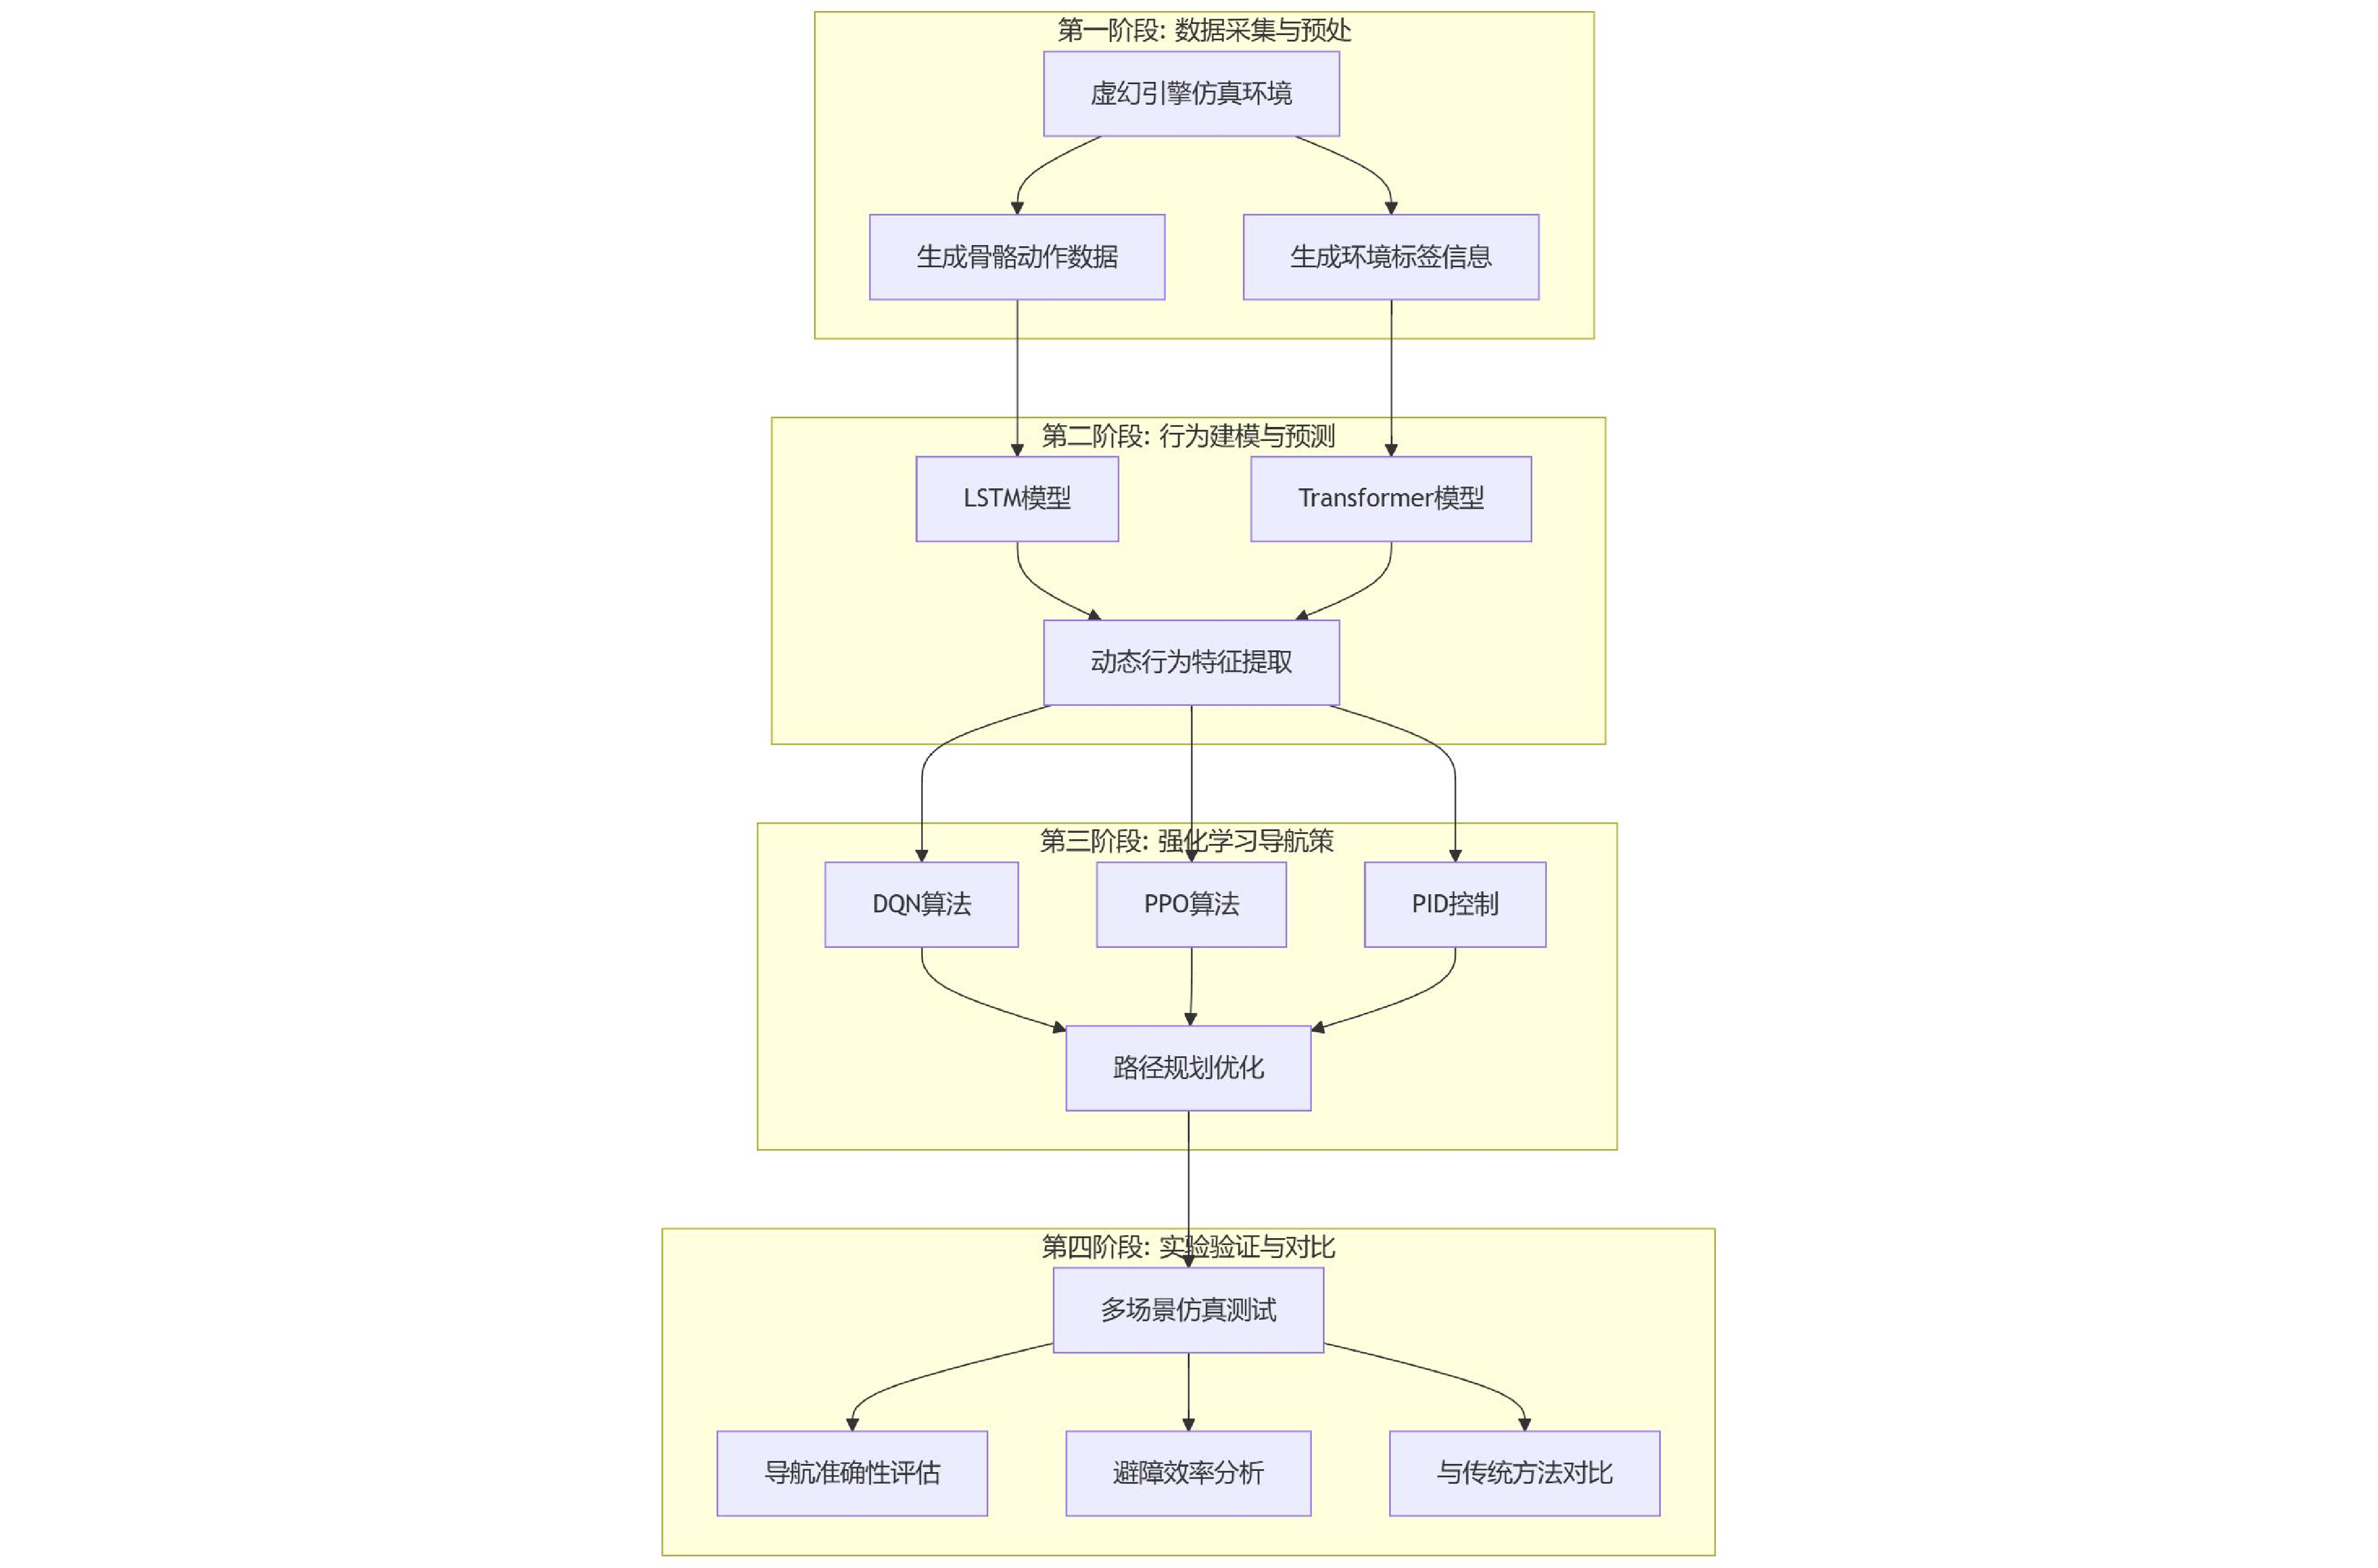
\includegraphics[width=0.8\textwidth]{sim/pedestrian/undergraduate/images/tech_route.pdf}
    \caption{本文技术路线}
    \label{fig:tech_route}
\end{figure}
